\chapter{Aufbau und Grundfunktionen}

Die PUMA-Einstiegsseite (~\autoref{fig:hauptmenü}) ist folgendermaßen aufgebaut:\\
1 -- \nameref{sec:suche}\\ 
2 -- \nameref{sec:spracheinstellung}\\
3 -- \nameref{sec:hauptmenue}\\
4 -- \nameref{sec:benutzermenue}\\
5 -- \nameref{sec:inhaltsbereich}\\
6 -- \nameref{sec:kontextmenue}\\ 

\begin{figure}[htb]
 \centering
 \fbox{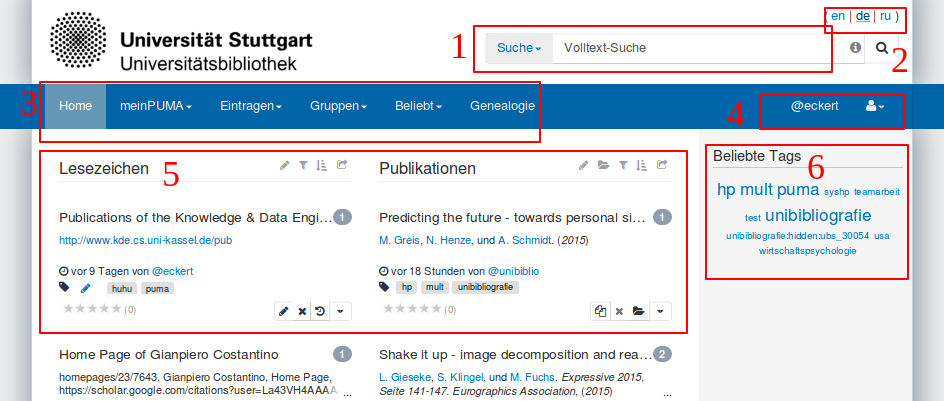
\includegraphics[width=12cm]{Bilder/Kapitel4/Puma_Hauptmenue}}
 \caption{Hauptmenü}
 \label{fig:hauptmenü}
\end{figure} 

\section{Suche}
\label{sec:suche}
Die Suche\index{Volltextsuche} (\textcolor{red}{1} in ~\autoref{fig:hauptmenü}) bietet die Möglichkeit, das System nach unterschiedlichen Kriterien zu durchsuchen. Standardmäßig werden alle Felder und Dateien durchsucht. Durch das Klicken auf das Dropdown-Menü \enquote{Suche}\index{Suche} lässt sich eingrenzen, in welchen Kategorien gesucht werden soll. Mit Hilfe von Suchsystemtags (\textit{sys:<Feldname><Feldwert>}) kann in Kategorien gezielt recherchiert werden (~\autoref{itm:suchSystemtag}).
 
\begin{figure}[h!]
 \centering
 \fbox{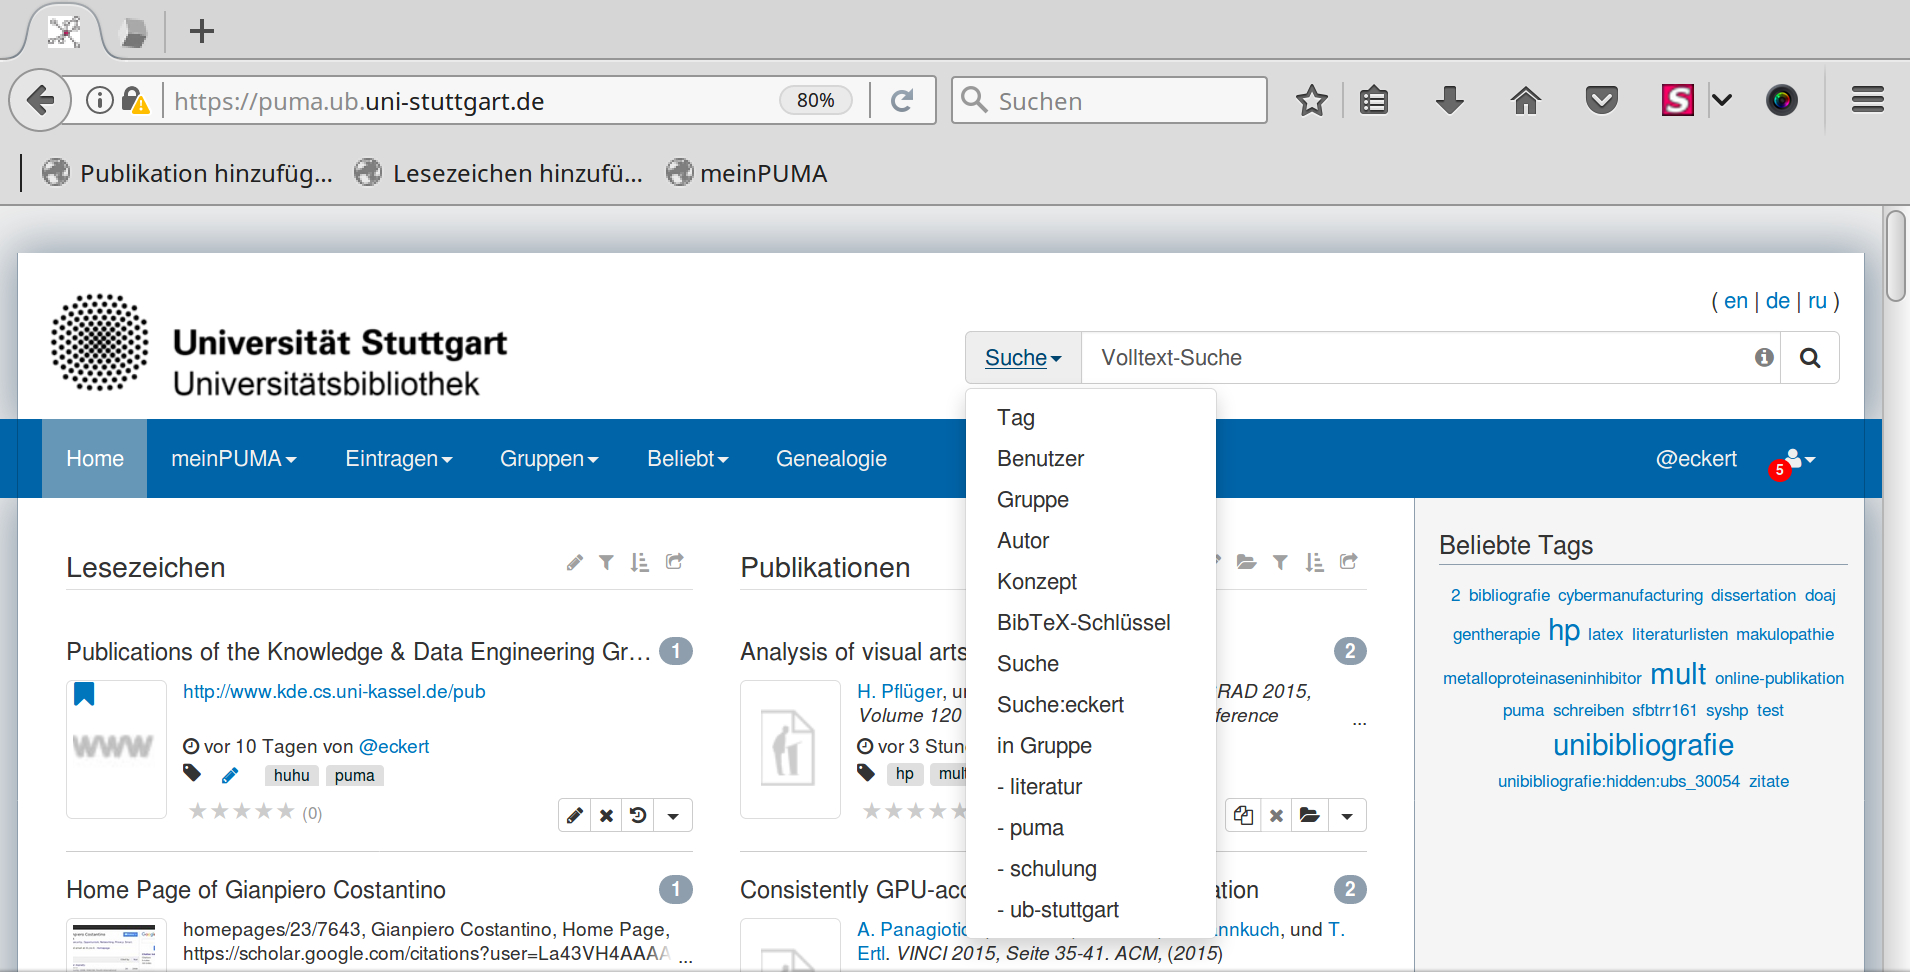
\includegraphics[width=10cm]{Bilder/Kapitel4/Suchleiste}}
 \caption{Suchleiste}
 \label{fig:suchleiste}
\end{figure} 

\section{Spracheinstellung}
\label{sec:spracheinstellung}
Die PUMA-Oberfläche kann in drei verschiedenen Sprachen (\textcolor{red}{2} in ~\autoref{fig:hauptmenü}) \index{Sprache} angezeigt werden:
Englisch (en), Deutsch (de) oder Russisch (ru)
%\begin{wrapfigure}{l}{5cm}
%\begin{mdframed}[style=tipp] \texttt{Einstellen der Standardsprache: Im Benutzermenü über den Reiter \enquote{Einstellungen} die Rubrik \enquote{Einstellungen} auswählen. Auf der erscheinenden Seite kann man die gewünschte Sprache festlegen. Die Änderung muss über \enquote{Layout speichern} bestätigt werden.}
%\end{mdframed}
\begin{tipp}
\texttt{Einstellen der Standardsprache: Im Benutzermenü über den Reiter \enquote{Einstellungen} die Rubrik \enquote{Einstellungen} auswählen. Auf der erscheinenden Seite kann man die gewünschte Sprache festlegen. Die Änderung muss über \enquote{Layout speichern} bestätigt werden.}
\end{tipp}
%\end{wrapfigure}
  

\section{Hauptmenü}
\label{sec:hauptmenue}
Nach dem Einloggen können über das Hauptmenü (\textcolor{red}{3} in ~\autoref{fig:hauptmenü}) wichtige Funktionen von PUMA ausgewählt werden:
\begin{itemize}
\item ~\nameref{subsec:home}
\item ~\nameref{subsec:meinPuma}
\item ~\nameref{subsec:eintragen}
\item ~\nameref{subsec:gruppen}
\item ~\nameref{subsec:beliebt}
\item ~\nameref{subsec:genealogie}
\end{itemize}

\subsection{Home\index{Home}}
\label{subsec:home}
Über das Menü \textit{Home} kann man jederzeit zurück auf die Startseite gelangen, auf der die neuesten Publikationen und Lesezeichen-Einträge angezeigt werden.

\subsection*{Mein PUMA\index{Mein PUMA}}
\label{subsec:meinPuma}
Mit den Standardeinstellungen \index{Funktionen!Einfache} können im Hauptmenü \textit{meinPUMA} im eingeloggten Modus folgende Untermenüs ausgewählt werden:
\begin{itemize}
\item meine Einträge\index{Einträge}: Eigenes Publikations- und Lesezeichenverzeichnis
\item diskutierte Einträge\index{Einträge!diskutierte}: Bewertungen von Publikationen und Lesezeichen, die selbst oder von anderen Nutzern an den eigenen Einträgen vorgenommenen wurden. 
\item verfolgte Einträge\index{Einträge!verfolgen}: Publikationen und Lesezeichen der Nutzer, denen man folgt (~\autoref{}) 
\item Einträge von Freunden\index{Einträge!von Freunden}: Einträge der befreundeten Nutzer werden angezeigt (~\autoref{}).
\end{itemize}
Im Benutzermenü können über \textit{Einstellungen} $\to$ Reiter \textit{Einstellungen} erweiterte Funktionen\index{Funktionen!Erweiterte} eingestellt werden. Das Menü wird um folgende Funktionen ergänzt:
\begin{itemize}
\item private Einträge\index{Einträge!privat}: Publikationen und Lesezeichen, die nur im eigenen Nutzerkonto sichtbar sind. 
\item Einträge für Freunde\index{Einträge!Freunde}: Einträge, die auch mit den befreundeten Nutzer geteilt werden.
\item Dokumente\index{Dokumente}: Übersicht über die angehängten Dokumente
\item Duplikate\index{Duplikate}: zeigt doppelte Einträge im eigenen Konto an
\item Konzepte\index{Konzepte}: Anzeige angelegter Konzepte (Gruppe von Schlagwörtern unter einem Supertag) (~\autoref{}). 
\item Lebenslauf\index{Lebenslauf}: Hier können persönliche Daten hinterlegt werden, die für andere Nutzer in PUMA sichtbar sind.
\item Publikationen durchstöbern: Mit dieser Funktion können eigene Lesezeichen und Publikationen dynamisch durch Auswahl von \tags und Autoren-Listen durchsucht werden. Zusätzlich gibt es Auswahl-Buttons für UND- oder ODER-Verknüpfungen.
\item BibTex\index{BibTex} exportieren: Exportiert alle Publikationen in der eigene Sammlung im BibTex-Format.
\end{itemize}

\subsection{Eintragen}
\label{subsec:eintragen}
\begin{enumerate}
    \item Lesezeichen eintragen\index{Lesezeichen!eintragen}: Ein neues Lesezeichen der eigenen Sammlung hinzufügen.  
    \item Publikation eintragen\index{Publikationen!eintragen}: Eine neue Publikation der eigenen Sammlung hinzufügen. 
    \item Lesezeichen importieren\index{Lesezeichen!Import}: Lesezeichen aus dem Browser oder Delicious (~\autoref{}) importieren.
    \item Publikationen importieren\index{Publikationen!Import}: Bestehende BibTeX- oder EndNote-Datei importieren.
\end{enumerate}

\subsection{Gruppen}
\label{subsec:gruppen}
Zeigt Funktionen zu Gruppen\index{Gruppen} an sowie die Gruppen in denen man Mitglied ist.
\begin{enumerate}
    \item Alle Gruppen: Überblick über alle existierenden Gruppen bei PUMA
    \item Eine neue Gruppe erstellen: eine eigene Gruppe kann erstellt werden (~\autoref{})
\end{enumerate}
\subsection{Beliebt\index{Beliebt}}
\label{subsec:beliebt}
Die drei häufigsten Einträge der letzten 7, 30 bzw. 120 Tage werden angezeigt.
\begin{enumerate}
    \item Einträge: Zeigt die beliebtesten Einträge an.
    \item \tags: Zeigt die beliebtesten \tags in einer Schlagwortwolke an. Je größer ein \tag ist, desto häufiger wird dieser verwendet.
    \item Autor: Zeigt die beliebtesten Autoren an.
    \item Konzepte: Zeigt die beliebtesten Konzepte und deren Zuordnungen an. 
    \item Diskussionen: Zeigt Lesezeichen und Publikationen an, über welche viel diskutiert wurde. 
\end{enumerate}
\subsection{Genealogie}
\label{subsec:genealogie}
Die PUMA Genealogie erstellt nutzerbasiert einen Stammbaum der Forschung an deutschen Universitäten. Ausgangspunkt ist der Dissertationskatalog der Deutschen Nationalbibliothek. Nutzerbasiert werden Beziehungen zwischen den an der Dissertation beteiligten Personen (Autor\_in, Betreuer\_in etc.) ergänzt.

\section{Benutzermenü}
\label{sec:benutzermenue}
\subsection{@username\index{@username}}
\label{subsec:username}
Über diesen Button gelangen Sie zu Ihrer Publikations- und Lesezeichensammlung. 
\subsection{Das Personensymbol}
\label{subsec:Personensymbol}
\begin{enumerate}
    \item Eingang\index{Eingang}: Dies ist Ihr Lesenzeichen-/~Publikations-Posteingang. Freunde/Gruppen können Ihnen Publikationen und Lesezeichen zuschicken, diese Eingänge landen dann hier.
    \item Ablage\index{Ablage}: In der Ablage können Sie aktuelle Literaturlisten zusammenstellen. 
    \item Freunde\index{Freunde}: Hier erhalten Sie einen Überblick über Ihre Freunde. 
    \item Tags bearbeiten\index{Tags!bearbeiten}: Hier können Sie Tags und Konzepte überarbeiten, beispielsweise alte Tags durch neue ersetzten. 
    \item Einstellungen\index{Einstellungen}: Zeigt Ihre persönlichen Benutzereinstellungen an. Sie können hier Ihr Profil, die allgemeinen Einstellungen, Ihren Lebenslauf sowie Einstellungen zu Gruppen ändern.
    \item Weblog\index{Weblog}: Leitet Sie zu dem Weblog\footnote{\url{http://blog.ub.uni-stuttgart.de/category/puma/}} von PUMA weiter.
    \item Hilfe\index{Hilfe}: Damit gelangen Sie zur Online-Hilfe.
    \item Abmelden\index{Abmelden}: Wenn Sie PUMA verlassen wollen, melden Sie sich hier ab. 
\end{enumerate}

\textbf{Der PUMA-Aufbau im Überblick}
%\small

\tabulinesep=1.5mm
\begin{longtabu}{|X[l]|X[l]|X[l]|X[l]|}\hline
\rowfont\bfseries
Hauptmenü & Untermenü & Reiter & Rubrik\\  \hline
\endfirsthead
\hline
%\multicolumn{4}{@{}l}{\small\dots\emph{Fortsetzung}}\\ \hline
\rowfont\bfseries
Hauptmenü & Untermenü & Reiter & Rubrik\\  \hline
\endhead
\hline
%\multicolumn{4}{@{}l}{\small\dots\emph{Fortsetzung nächste Seite} \ldots}\\ \hline
\endfoot
%\hline
\endlastfoot
Eintragen&Lesezeichen eintragen &- &-\\ \cline{2-4}
&Publikation eintragen &Per Hand& Tragen Sie Ihre Publikation hier ein\\\cline{3-4}
&&BibTex/EndNote-Schnipsel& Tragen Sie hier Ihre BibTex- oder EndNote-Schnipsel ein\\ \cline{4-4}
&&& Einstellungen\\ \cline{3-4}
&&Datei hochladen& Laden Sie ihre BibTex- oder EndNote-Datei hier hoch\\ \cline{4-4}
&&&Einstellungen\\ \cline{3-4}
&&ISBN/DOI& ISBN\\ \cline{4-4}
&&& ISSN \\ \cline{4-4}
&&&DOI\\ \cline{3-4}
&&Code scannen&-\\ \cline{2-4}
&Lesezeichen importieren&- &Importieren Sie Ihre Lesezeichen aus Ihrem Browser\\ \cline{4-4}
&& & Importieren Sie Ihre Delicious Daten\\ \cline{2-4} 
&Publikationen importieren &-&-\\ \hline
Gruppen&Alle Gruppen& Gruppen von A-Z &-\\ \cline{2-4}
&Gruppen, in denen der Nutzer Mitglied ist& Einträge &-\\\cline{3-4}
&&Interessant für &- \\ \cline{3-4}
&&Sichtbar&-\\ \cline{3-4}
&&Dokumente&-\\ \cline{3-4}
&&diskutierte Einträge&-\\ \cline{3-4}
&&Einstellungen&Gruppeneinstellungen und Mitgliederliste\\ \cline{2-4}
&Eine neue Gruppe erstellen&-&-\\ \hline
Personensymbol&Eingang&-&-\\ \cline{2-4}
&Ablage&-&-\\ \cline{2-4}
&Freunde&Ihre Freunde&- \\ \cline{3-4}
&&Sie sind ein Freund von&- \\ \cline{2-4}
&Tags bearbeiten&-&Umbenennen/ Ersetzen von Tags\\ \cline{4-4}
&&&Subtags zu Konzepten hinzufügen\\ \cline{4-4}
&&&Subtags von Konzept löschen\\ \cline{2-4}
&Einstellungen&Mein Profil&Allgemeine Informationen\\ \cline{4-4}
&&&Kontakt\\ \cline{4-4}
&&&Über mich\\ \cline{4-4}
&&&Ein Bild für meinen Lebenslauf\\\cline{3-4}
&&Einstellungen&Layouts Ihrer Tagbox und Ihrer Eintragsbilder\\\cline{4-4}
&&&API\\\cline{4-4}
&&&Logging und Löschen\\\cline{4-4}
&&&Passwort ändern\\\cline{4-4}
&&&Mein Konto löschen\\\cline{3-4}
&&JabRef Layout-Datei&-\\\cline{3-4}
&&Lebenslauf& Lebenslauf editieren\\\cline{4-4}
&&&Layout editieren\\ \cline{4-4}
&&&Vorschau wird erzeugt\\\cline{3-4}
&&OAuth-Consumers&- \\\cline{3-4}
&&Gruppen&Eine neue Gruppe erstellen\\\cline{4-4}
&&&Gruppen\\\cline{2-4}
&Einstellungen&Synchronisation&-\\\cline{2-4}
&Weblog&-&-\\\cline{2-4}
&Hilfe&-&-\\\cline{2-4}
&Abmelden&-&-\\\hline
\caption{Der PUMA-Aufbau im Überblick}
\label{tab:pumaAufbau}
\end{longtabu}

%\normalsize

\section{Inhaltsbereich}
\label{sec:inhaltsbereich}
Hier sehen Sie die aktuellsten Lesezeichen und Publikationen von Ihnen und anderen Nutzern. 
\section{Kontextmenü}
\label{sec:kontextmenue}
Auf der Einstiegsseite werden die beliebtesten Tags\index{Tags} angezeigt. In den Einstellungen kann zwischen der Wolken- oder Listen-Ansicht gewählt werden.